\documentclass{article}
\usepackage{graphicx} % Required for inserting images
\usepackage{tcolorbox} % Required for the colored box
\usepackage{caption}
\usepackage{verbatim}
\usepackage{listings}

% Define a custom command for section headings
\newcommand{\heading}[1]{\noindent\textcolor{gu-green}{\textbf{\large #1}}}

\begin{document}

\begin{titlepage}
  \begin{center}
  
    
    % Insert the university logo
    
\includegraphics[width=0.4\textwidth]{logo.svg.png}
    
    {\LARGE\textbf{Green University of Bangladesh}}\\
    \vspace{0.5cm}
    {\Large Department of Computer Science and Engineering}\\
    \vspace{1cm}
    
    \rule{\linewidth}{0.5mm}
    
    \vspace{0.5cm}
    {\LARGE\textbf{Lab Report-02}}\\
    \vspace{0.5cm}
    {\Large Course Title: Object Oriented Programming Lab}\\
    \vspace{0.2cm}
    {\Large Course Code: CSE-221 Section: DA}\\
    \vspace{0.5cm}
   \rule{\linewidth}{0.5mm}
 
    \LARGE \textbf{} Experiment Title : Transposing and Summation a 3D Matrix in Java  \newline
   
     \LARGE \textbf{} Semester: \LARGE Spring, Year: 2023\\
    \vspace{0.5cm}
    \LARGE \textbf{} Program: B.Sc in CSE (Day)\\
    
    \vspace{3cm}
    \begin{tcolorbox}[colback=white,colframe=black,width=10cm,height=2cm]
      \LARGE{Student Name:} IBRAHIM REFAT \\
      \textbf{ID:} 221902333 \\
    \end{tcolorbox}
    
    \vspace{2cm}
    \textbf{Lab Date:} 01/03/2023 \\
    \vspace{0.2cm}
  \textbf{Submission Date:} 03/03/2023 \\
    \vspace{0.2cm}
   \textbf{Course Teacher:} Dr. Muhammad Aminur Rahaman
    
  \end{center}
\end{titlepage}

% Start the main content on a new page
\clearpage

\section{Title}
\Large 01. Implement transposing and Summation 3D Matrix \newline
\
\section{Objective}
\large 1. Through this problem, I have gained a solid understanding of matrices, 3D matrices, matrix transposition, and addition using for loops. This lab exercise has greatly improved my ability to work with for loops.

\section{Procedure}
\Large Problem : 01
\begin{enumerate}
\item Start
\item Take input from user for dimensions .
\item Create a 3D matrix of dimensions.
\item Take input from user for the values of each element of the 3D matrix.
\item Print the 3D matrix.
\item Create another 3D matrix of dimensions.
\item Take input from user for the values of each element of the second 3D matrix.
\item Transpose the first 3D matrix using three nested for loops.
\item Transpose the second 3D matrix using three nested for loops.
\item After complete transposing do summation them.
\item Print the sum of the two matrices.
\item Exit

\end{enumerate}


\begin{enumerate}
    \item 
    
\end{enumerate}


\section{Implementation}
{ \textbf{Problem : 01}}
\begin{lstlisting}[language=Java, breaklines=true]
import java.util.Scanner;

public class ThreeDmatrixTransposeAndSum {

    public static void main(String[] args) {
        Scanner scan = new Scanner(System.in);
        int size;
        System.out.print("Enter size of matrix : ");
        size = scan.nextInt();
        int [][][]Sum = new int [size][size][size];
        System.out.println("Enter "+size*size*size+" elements for first matrix :");
        int[][][] matrix1 = new int[size][size][size];
        for (int i = 0; i < size; i++) {
            for (int j = 0; j < size; j++) {
                for (int k = 0; k < size; k++) {
                    matrix1[i][j][k] = scan.nextInt();
                }
            }
        }
        
        int[][][] transposedMatrix1 = transpose(matrix1, size);
        
        System.out.println("Enter "+size*size*size+" elements for second matrix :");
        int[][][] matrix2 = new int[size][size][size];
        for (int i = 0; i < size; i++) {
            for (int j = 0; j < size; j++) {
                for (int k = 0; k < size; k++) {
                    matrix2[i][j][k] = scan.nextInt();
                }
            }
        }
        
        int[][][] transposedMatrix2 = transpose(matrix2, size);
        
        System.out.println("The summation of transpose matrix A & B");
        
        for(int i=0;i<size;i++)
        {
            for(int j=0;j<size;j++)
            {
                for(int k=0;k<size;k++)
                {
                    Sum[i][j][k] = transposedMatrix1[i][j][k]+transposedMatrix2[i][j][k];
                    System.out.print(Sum[i][j][k] + " ");
                }
                System.out.println();
            }
            System.out.println();
        }
    }
    
    public static int[][][] transpose(int[][][] matrix, int n) {
    int[][][] transpose = new int[n][n][n];
    System.out.println("The transpose matrix is : ");
    for (int i = 0; i < n; i++) {
        for (int j = 0; j < n; j++) {
            for (int k = 0; k < n; k++) {
                transpose[i][j][k] = matrix[i][k][j];
                System.out.print(transpose[i][j][k] + " ");
            }
            System.out.println();
        }
        System.out.println();
    }
    return transpose;
}

}
\end{lstlisting}


\section{Test Result}
\large \textbf{01}
 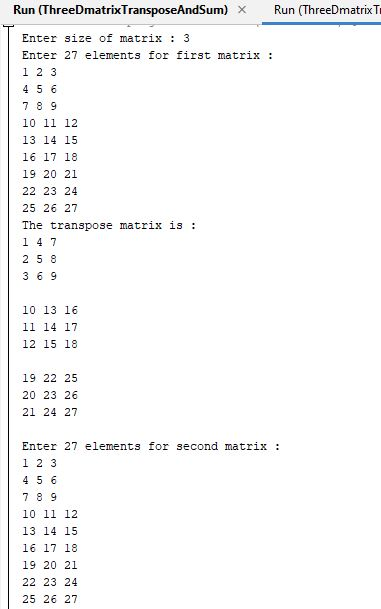
\includegraphics[width=1\textwidth]{terminal1.JPG}
 \centering
\large Figure 01 : Transposing and Summing
\vspace{0.5cm}

\large \textbf{02}
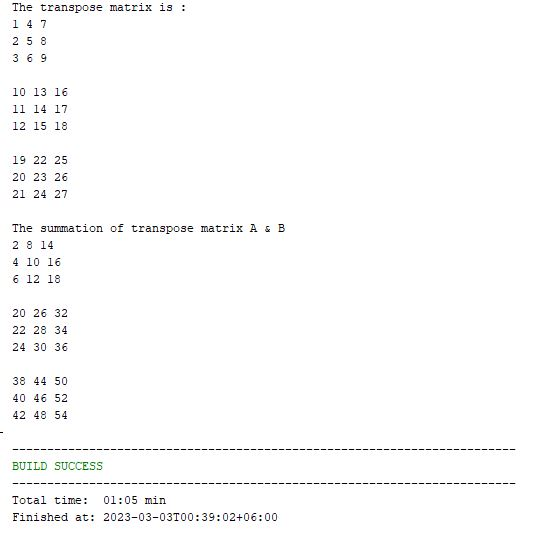
\includegraphics[width=1\textwidth]{terminal2.JPG}
 \centering
 


 
\section{ANALYSIS AND DISCUSSION}
 This problem challenged me to work with matrices and overcome errors. I deepened my understanding of 3D arrays and learned that we can work with up to 4 dimensions. This experience improved my problem-solving skills and expanded my array knowledge, benefitting future programming projects. which will undoubtedly benefit me in future programming endeavors.
  

 

\end{document}